\section{Mehr Java} 
\subsection{Wrapper}
\begin{frame}[fragile]
	\frametitle{Wrapperklassen}
\huge Wrapperklassen
\end{frame}

\begin{frame}[fragile]
	\frametitle{Wrapperklassen}
	\begin{columns}
		\begin{column}{0.5\textwidth}
			\small
			\begin{itemize}
			  \item Verpacken primitive Datentypen in Objekte
			  \item F\"ur Situationen in denen Objekte ben\"otigt 
			  werden\\
			  Beispielsweise Collections
			  \item Wrapper im Package ''java.lang''
			\end{itemize}
		\end{column}
		\begin{column}{0.5\textwidth}
			\begin{table}
				\begin{small}
					\begin{tabular}{l|l}
					Wrapper & Datentyp \\ \hline
					Byte & byte \\
					Short & short \\
					Integer & int \\ 
					Long & long \\
					Float & float \\
					Double & double \\
					Boolean & boolean \\
					Character & char \\
					Void & void
					\end{tabular}
				\end{small}
			\end{table}
		\end{column}
	\end{columns}
\end{frame}

\begin{frame}[fragile]
	\frametitle{Wrapperklassen}
	\begin{columns}
		\begin{column}{0.5\textwidth}
			\small
			\begin{itemize}
			  \item Wrapper enthalten Attribut vom Datentyp
			  \item Es existieren verschiedene Konstruktoren\\
			  (Parameter: Datentyp, String\ldots)
			  \item K\"onnen prim. Datentyp via Methoden
			  zur\"uckliefern
			  \item Es existieren static-Methoden zur Konvertierung
			\end{itemize}
		\end{column}
		\begin{column}{0.5\textwidth}
			\begin{lstlisting}
				// Konstruktor mit prim. Typ
				Short myShort = new Short((short) 5);
				
				// Konstruktor mit String
				Short myShort2 = new Short("5");
				
				//Prim. Typ zurueckholen
				short s = myShort.shortValue();
				
				//Oder als String
				String shortString = myShort.toString();
				
				// Konvertierung von String in short
				short ps = Short.parseShort("5");
				
				// Konvertierung von String 
				// in Short-Objekt
				Short vs = Short.valueOf("5");
			\end{lstlisting}
		\end{column}
	\end{columns}
\end{frame} 

\begin{frame}[fragile]
	\frametitle{Autoboxing bei Wrapperklassen}
	\begin{columns}
		\begin{column}{0.5\textwidth}
			\small
			\begin{itemize}
			  \item Umwandlung zwischen prim. Datentyp und 
			  Wrapper nimmt Compiler automatisch vor
			  \item Name dieser Funktion: Autoboxing
			\end{itemize}
		\end{column}
		\begin{column}{0.5\textwidth}
			\begin{lstlisting}
				// Array mit Integer-Objekten
				Integer[] meineInts = new Integer[5];
				
				// Primitiver Typ ins Objekt-Array
				meineInts[0] = 5;
				
				// Objekt in prim. Typ gepackt
				int erster = meineInts[0];
			\end{lstlisting}
		\end{column}
	\end{columns}
\end{frame}

\subsection{Innere Klassen}
\begin{frame}[fragile]
	\frametitle{Innere Klassen}
	\huge Innere Klassen
\end{frame}

\begin{frame}[fragile]
	\frametitle{Innere Klassen}
	\begin{columns}
		\begin{column}{0.5\textwidth}
			\small
			\begin{itemize}
			  \item Innere Klassen sind in Klassen 
			  definierte Klassen
			  \item Inner-Class hat Zugriff auf alle
			  Attribute der Outer-Class
			  \item Outer-Class hat Zugriff auf alle
			  Attribute der Inner-Class
			  \item Outer-Class kann Objekt der Inneren 
			  instanziieren
			\end{itemize}
		\end{column}
		\begin{column}{0.5\textwidth}
			\begin{lstlisting}
			// Aeussere Klasse
			public class Outer {
				private final int out = 5;
				private final Inner innen = new Inner();
									
				// Innere Klasse
				public class Inner {
					int out;
					private int whatsOut() {
						// Outer.this da
						// das innere ''out''
						// das aeussere ueberdeckt
						// ansonsten: return out;
						return Outer.this.out;
					}
				}
				
				public static void main(String[] args) {
					// Instanz von Outer-Class
					Outer o = new Outer();
											
					// Zugriff auf Private-Konstrukte 
					// Was passiert wenn folgende 
					// Zeile nicht in Outer steht? 
					// z.B. in einer anderen Klasse?
					o.innen.whatsOut();
				}
			}
			\end{lstlisting}
		\end{column}
	\end{columns}
\end{frame}

\begin{frame}[fragile]
	\frametitle{Zugriff auf Inner-Classes von au"sen}
	\begin{columns}
		\begin{column}{0.5\textwidth}
			\small
			\begin{itemize}
			  \item Ist innere Klasse nicht private,
			  kann auch au"serhalb von Outer darauf 
			  zugegriffen werden
			  \item Wichtig: Objekt von Outer-Class
			  \item Inner-Objekt ist an Outer-Objekt
			  gebunden
			\end{itemize}
		\end{column}
		\begin{column}{0.5\textwidth}
			\begin{lstlisting}
				// Outer Objekt
				Outer o = new Outer();
				
				// Inner kann nun wie normales
				// Objekt genutzt werden
				Inner inner = o.new Inner();
			\end{lstlisting}
		\end{column}
	\end{columns}
\end{frame}

\begin{frame}[fragile]
	\frametitle{Weitere Eigenschaften von inneren Klassen}
		\begin{itemize}
		  \item Innere Klassen k\"onnen auch in Methoden
		  definiert werden\\
		  Dann hat innere Klasse Zugriff auf ''final''
		  Variablen der \"Au"seren
		  \item Oftmals Einsatz in GUIs zur Ereignisbehandlung
		  \item Zur mehrfachen Implementierung von Interfaces
		  in einer Klasse
		\end{itemize}
\end{frame}

\subsection{Anonyme Klassen}
\begin{frame}[fragile]
	\frametitle{Anonyme Klassen}
	\huge Anonyme Klassen
\end{frame}

\begin{frame}[fragile]
	\frametitle{Anonyme Klassen}
	\begin{columns}
		\begin{column}{0.5\textwidth}
			\begin{itemize}
				  \item Haben keinen Klassennamen
				  \item Wird dort definiert wo 
				  ''new'' aufgerufen wird
				  \item Z.B. zur Implementierung von Interfaces\\
				  (Listener etc\ldots)
				  \item Kann wie normales Objekt benutzt werden
			\end{itemize}
		\end{column}
		\begin{column}{0.5\textwidth}
			\begin{lstlisting}
				Melkbar m = 
					// In den Klammern koennen Parameter
					// fuer Konstruktoren stehen
					new Melkbar(){
						public int gebeMilch(){
							return 5;
						}
					};
			\end{lstlisting}
		\end{column} 
	\end{columns}
\end{frame}

\subsection{Ausnahmen}
\begin{frame}[fragile]
	\frametitle{Ausnahmen}
	\huge Ausnahmen
\end{frame}

\begin{frame}[fragile]
	\frametitle{Exceptions}
	\begin{itemize}
	  \item Zur kontrollierten Fehlerbehandlung
	  \item Damit nicht direkt das Programm abbricht
	  \item Dazu werden Exceptions erzeugt und im Fehlerfall
	  geworfen
	  \item Exceptions = Ausnahme = Fehlerobjekt
	  \item Exception ist vom Typ ''throwable''
	\end{itemize}
\end{frame}

\begin{frame}[fragile]
	\frametitle{Exceptions}
	\begin{itemize}
	  \item try-catch kann Exceptions fangen
	  \item Exception ist ein ''Throwable''
	  \item Es wird zwischen ''Unchecked Exceptions''
	  und ''Checked Exceptions'' Exceptions unterschieden
	  \item ''Unchecked Exceptions'' erben von RuntimeException
	  \item Durch erben von ''Exception'' k\"onnen
	  eigene Ausnahmen gebaut werden
	\end{itemize}
\end{frame}  

\begin{frame}[fragile]
	\frametitle{Exception-Hierarchie}
	\center
	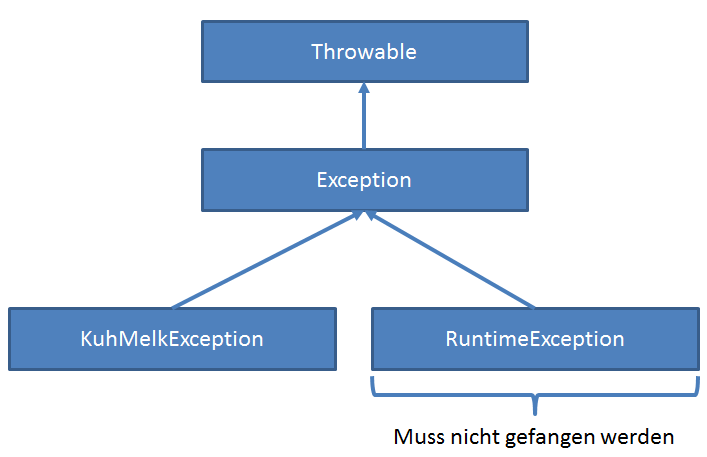
\includegraphics[width=1\textwidth,
	keepaspectratio=true]{bilder/exceptions.png}
\end{frame}

\begin{frame}[fragile]
	\frametitle{Exception-Hierarchie}
	\begin{columns}
		\begin{column}{0.5\textwidth}
			\small
			\begin{itemize}
			  \item Methoden muss mit ''throws'' zeigen dass sie eine Exception 
			  werfen kann 
			  \item Mit ''throw'' wird Exception geworfen
			  \item Bei RuntimeExceptions wird kein ''throws'' im
			  Methodenkopf ben\"otigt
			\end{itemize}
		\end{column}
		\begin{column}{0.5\textwidth}
			\begin{lstlisting}
				public int gebeMilch() 
					// Methode kann Exception werfen
					throws KuhMelkException{
					if(milch == 0){
						// Exceptoin erzeugen
						throw new KuhMelkException("Milch leer");
					}
					return milch;
			}
			\end{lstlisting}
		\end{column}
	\end{columns}
\end{frame}

\begin{frame}[fragile]
	\frametitle{Exceptions behandeln}
	\begin{columns}
		\begin{column}{0.5\textwidth}
			\small
			\begin{itemize}
			  \item 2 M\"oglichkeiten im Umgang mit
			  Exceptions:
			  \begin{enumerate}
			    \item Try-Catch
			    \item Wiederrum ein Throws in aufrufende
			    Methode
			  \end{enumerate}
			  \item In Catch kann auch geworfen werden
			  \item Mit mehreren Catch-Bl\"ocken k\"onnen
			  mehrere Exception-Typen gefangen werden
			  \item Methode kann mehrere Exception-Typen
			  werfen
			\end{itemize}
		\end{column}
		\begin{column}{0.5\textwidth}
			\begin{lstlisting}
				// try-catch
				try {
					meinMelkbar.gebeMilch();
				} catch (KuhMelkException k){
					// Code zur Fehlerbehandlung
					System.out.println(k.getMessage());
				} finally {
					// Wird immer ausgefuehrt
					// z.B. Kuh Herausbringen
				}
				
			\end{lstlisting}
		\end{column}
	\end{columns}
\end{frame}

\subsection{GUIs und Grafik} 
\begin{frame}[fragile]
	\frametitle{Swing}
	\huge Swing
\end{frame} 

\begin{frame}[fragile]
	\frametitle{Swing}
	\begin{itemize}
	  \item Im Gegensatz zu AWT (Abstract Windowing Toolkit)
	  sorgt Swing f\"ur einheitliches Look-and-Feel
	  \item Swing verwendet JFrames zur Fensterdarstellung
	  \item JFrame hat ''ContentPane'', ein Container f\"ur
	  Komponenten
	\end{itemize}
\end{frame}

\begin{frame}[fragile]
	\frametitle{Ein erstes Fenster}
	\begin{columns}
		\begin{column}{0.5\textwidth}
			\small
			\begin{itemize}
			  \item F\"ur ein neues Fenster leiten wir von JFrame ab
			  \item Konstruktor unserer Klasse:
			  	\begin{enumerate}
			  	  \item super(''Erstes Fenster'');
			  	  \item setSize(100,100);
			  	  \item setVisible(true);
			  	  \item \ldots
			  	\end{enumerate}
			\end{itemize}
		\end{column}
		\begin{column}{0.5\textwidth}
			\begin{lstlisting}
				// MeinFenster erbt von JFrame
				public class MeinFenster extends JFrame {
					MeinFenster() {
						// Konstruktor von JFrame
						// Fuer den Titel
						super("Erstes Fenster");
						
						// Groesse des Fenster
						setSize(100, 100);
						
						// Fenster sichtbar machen
						setVisible(true);
						
						// Bestimmen was beim Schliessen
						// des Fensters passiert
						setDefaultCloseOperation(EXIT_ON_CLOSE);
					}
					
					public static void main(String[] args){
						MeinFenster fenster = new MeinFenster();
					}
				}
			\end{lstlisting}
		\end{column}
	\end{columns}
\end{frame}  

\begin{frame}[fragile]
	\frametitle{Grafik}
	\huge Grafik
\end{frame} 

\begin{frame}[fragile]
	\frametitle{Zeichnen mit Graphics}
	\begin{columns}
		\begin{column}{0.5\textwidth}
			\small
			\begin{itemize}
			  \item Zum zeichnen \"uberschreiben wir die
			  Paint-Methode aus JFrame
			  \item Paint-Methode:
			  	\begin{enumerate}
			  	  \item K\"ummert sich um Ausgabe
			  	  \item Automatischer Aufruf bei Neuzeichnung
			  	  des Inhalts
			  	  \item Wird nicht vom Entwickler aufgerufen,
			  	  daf\"ur ist Repaint
			  	  \item Parameter: Graphics-Objekt
			  	\end{enumerate}
	\end{itemize}
	\end{column}
		\begin{column}{0.5\textwidth}
			\begin{lstlisting}
				public class MeinFenster extends JFrame {
					MeinFenster() {
						super("Erstes Fenster");
						setSize(100, 100);
						setVisible(true);
						setDefaultCloseOperation(EXIT_ON_CLOSE);
					}
					
					// Die Paint-Methode
					// Aufruf vom Entwickler nur!  
					// durch Repaint
					public void paint(Graphics g){
						// Mit Graphics-Objekt kann man zeichnen
						g.fillRect(20,20,50,50);
					}
					
					public static void main(String[] args){
						MeinFenster fenster = new MeinFenster();
					}
				}
			\end{lstlisting}
		\end{column}
	\end{columns}
\end{frame}

\begin{frame}[fragile]
	\frametitle{Zeichnen mit Graphics}
	\begin{columns}
		\begin{column}{0.4\textwidth}
			\small
			\begin{itemize}
			  \item Graphics dient der grafischen Ausgabe
			  \item Verwaltet Farbe und Schriftart
			  \item Farbdarstellung mit der Klasse ''Color''
			  \item Schriftart wird durch die Klasse ''Font''
			  definiert (Schriftart f\"ur drawString(\ldots))
	\end{itemize}
	\end{column}
		\begin{column}{0.6\textwidth}
			\begin{lstlisting}
				public class MeinFenster extends JFrame {
					MeinFenster() {
						super("Erstes Fenster");
						...
					}
					
					// Die Paint-Methode
					// Niemals selbst aufrufen NUR  
					// durch Repaint
					public void paint(Graphics g){
						// Mit Graphics-Objekt kann man zeichnen
						g.fillRect(20,20,50,50);
						
						// Farbe setzen
						g.setColor(Color.GREEN)
						
						// Wieder zeichnen
						g.drawLine(5,5,100,100);
						
						// Font erstellen und setzen
						Font f = new Font("Serif", Font.BOLD, 12);
						g.setFont(f);
						
						// Schreiben
						g.drawString("Hallo", 20,20);
					}
					...
				}
			\end{lstlisting}
		\end{column}
	\end{columns}
\end{frame}

\begin{frame}[fragile]
	\frametitle{Fonts}
		\begin{center}
			\begin{itemize}
			  \item Konstruktor:\\
			  new Font(String name, int style, int size)
			  \item 5 Schriftarten = Name
			  \item 3 Stile = style
			\end{itemize}
		\end{center}
	\begin{columns}
		\begin{column}{0.5\textwidth}
			\begin{table}
			\begin{tabular}{l}
			 Schriftarten \\ \hline
			SansSerif\\
					Serif\\
					Monospaced\\
					Dialg\\
					DialogInput
			\end{tabular}
			\end{table}
		\end{column}
		\begin{column}{0.5\textwidth}
			\begin{table}
			\begin{tabular}{l|l}
			Style & Bedeutung \\ \hline
					Font.PLAIN & Normal\\
					Font.BOLD & Fett\\
					Font.ITALIC & Kursiv
			\end{tabular}
			\end{table}
		\end{column}
	\end{columns}
\end{frame}

\begin{frame}[fragile]
	\frametitle{Event-Handling}
	\huge Event-Handling
\end{frame} 

\begin{frame}[fragile]
	\frametitle{Events}
	\begin{itemize}
	  \item Bei Programmierung (insbesondere GUI)
	  existiert eine F\"ulle wichtiger Ereignisse
	  \item Ereignisse haben eine Quelle
	  \item Um Ereignis mitzubekommen kann Objekt
	  sich bei Quelle registrieren
	  \item Quelle informiert dann bei \"Anderung
	  \item Welches Entwurfsprinzip entspricht diesem Muster?
	\end{itemize}
\end{frame} 

\begin{frame}[fragile]
	\frametitle{Listener}
	\begin{itemize}
	  \item Bei Quelle registrierte Objekte hei"sen Listener
	  \item Dazu implementiert Empf\"anger eine Schnittstelle\\
	  ein ''Listener-Interface''
	\end{itemize}
	\small
	\begin{table}
	\begin{tabular}{l|l|l}
	Listener & Registrierung & Quelle\\ \hline
			ActionListener & addActionListener & Button\ldots\\
			MouseListener & addMouseListener & Component\\
			MouseMotionListener & addMouseMotionListener & Component\\
			\ldots & \ldots & \ldots
	\end{tabular}
	\end{table}
\end{frame} 

\begin{frame}[fragile]
	\frametitle{Ereignisobjekte}
	\begin{columns}
		\begin{column}{0.4\textwidth}
			\small
			\begin{itemize}
			  \item Ereignis wird durch Objekt repr\"asentiert
			  \item Ereignisobjekte beziehen sich auf die Art 
			  des Ereignisses (ActionEvent, MouseEvent \ldots)
			  \item Bei Event wird Event-Objekt erzeugt und an
			  Listener \"ubergeben
			\end{itemize}
		\end{column}
		\begin{column}{0.6\textwidth}
			\begin{lstlisting}
				public class Fenster extends JFrame {
					Fenster() {
						super("test");
						setDefaultCloseOperation(EXIT_ON_CLOSE);
						setSize(400, 400);
						setLocation(100, 100);
						addMouseListener(new MeinMouseListener());
					}
									
					// Listener als Inner-Class
					private class MeinMouseListener implements MouseListener {
					...
					@Override
					public void mousePressed(MouseEvent e) {
						Graphics g = Fenster.this.getGraphics();
						// Event hat Attribute wie x und y						   
						g.fillRect(e.getX(), e.getY(), 2, 2);
					}
					...
					}
									
					public static void main(String[] args) {
						Fenster f = new Fenster();
						f.setVisible(true);
					}
				}
			\end{lstlisting}
		\end{column}
	\end{columns}
\end{frame}

\begin{frame}[fragile]
	\frametitle{GUI}
	\huge GUI
\end{frame} 

\begin{frame}[fragile]
	\frametitle{GUI}
	\begin{itemize}
	  \item Anordung von Interaktionselementen in einem Fenster
	  	\begin{enumerate}
	  	  \item Buttons
	  	  \item Radio-Buttons
	  	  \item Check-Boxen
	  	  \item Textfields
	  	  \item Label
	  	\end{enumerate}
	  \item Diese Elemente sind Komponenten
	  \item Sie erben alle von der Klasse Component
	\end{itemize}
\end{frame}

\begin{frame}[fragile]
	\frametitle{GUI}
	\begin{itemize}
	  \item Anordnung der Komponenten \"uber Layoutmanager
		  \begin{enumerate}
		  	  \item Border-Layout-Manager
		  	  \item Flow-Layout-Manager
		  	  \item Grid-Layout-Manager
		  	\end{enumerate}
	  \item Lassen sich mit JPanels auch verschachteln
	\end{itemize}
\end{frame} 

\begin{frame}[fragile]
	\frametitle{GUI}
	\begin{columns}
		\begin{column}{0.5\textwidth}
			\small
			\center
			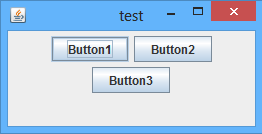
\includegraphics[width=0.8\textwidth,
			keepaspectratio=true]{bilder/layouts.png}
		\end{column}
		\begin{column}{0.5\textwidth}
			\begin{lstlisting}
				// 1. Borderlayout fuer das Fenster
				BorderLayout border = new BorderLayout();
				this.getContentPane().setLayout(border);
				
				// Panel
				JPanel p = new JPanel();
				
				// 2. Layout fuer das JPanel
				p.setLayout(new FlowLayout());
				
				// Button fuer das Panel
				JButton button = new JButton("Button1");
				JButton button2 = new JButton("Button2");
				JButton button3 = new JButton("Button3");
				p.add(button); 
				p.add(button2);
				p.add(button3);
				
				// Panel der Contentpane hinzufuegen
				this.getContentPane().add(p, BorderLayout.CENTER);
			\end{lstlisting}
		\end{column}
	\end{columns}
\end{frame}